\section{FRAMEWORK UMBRELLA ARCHITECTURE AND DESIGN}
%This is a summary of section 2 in the Hoffman paper

A hierarchical trust analysis can look at the entire system and combine measurements from multiple sources, making
it more powerful than measuring a single component or layer.
This section discusses a comprehensive mechanism that provides a scalable and extendable methodology of trust
 evaluation and analysis which is implemented on Android-based mobile devices. \weiss{why is it limited to Android?}
Trust evaluation of a mobile smartphone device is a complex subject, which depends on multiple characteristics, 
e.g. sensor accuracy, the rate of encrypted messages, and/or the probability of a system's breakdown over a given period of time. Its evaluation should integrate various metrics ranging from the accuracy and reliability of the data sources to the security of the procedures and tools used. The major research challenge of the framework design is integrating the numerous metrics needed to characterize a device's trustworthiness while working with limited resources and processing power. 
We address this challenge by hierarchically structuring the composition of trust metrics as well as by designing a specialized calculus to evaluate the overall trust metric. 
Therefore, the major innovative emphasis in our framework design is put on the integration of a wide variety of indicators and their evaluation procedures. The framework procedures output the overall trust evaluation indicators and additionally calculate the individual product of metrics characterizing system features which are then used to produce recommendations for improvement. The trust evaluation will facilitate decision-making, improve performance and increase accountability through the collection, analysis, and reporting of relevant performance-related data. This design facilitates the framework extension through
 the inclusion of other metrics, as well as the ease of modification and improvement (see fig~\ref{})
Current implementation of this framework provides the following metric functionality: 

\begin{enumerate}
\item Analysis of the installed applications through the application-specific metadata provided by the Play store. Applications represent the largest security and privacy risk to a device and user's data. The data provided by the Play store leverages the experiences of millions of users and holds all data associated with the distribution of an application including its associated documentation. The Play store also provides meta-information about applications which gives useful characteristic data about an application. These data can be used to assess an individual application's risk. Rules were generated to classify each application into a risk impact class based on this meta-data. The combined trust classes of all applications installed on a device would be used to create a security risk rating for the whole device.

\item The usage verification of security tools embedded into the operating system and proper preventative security practices. Android provides users with many different tools which increase the security and privacy of their devices in addition to updates to patch exposed vulnerabilities. When properly used, these tools improve the security of the devices. In order to gather a comprehensive overview of the software running on a mobile device an analysis of the operating system and user settings is performed. First the operating system is checked to confirm that it is running the most recent version available. Second the personal security settings on the device are examined to determine if the user is utilizing the appropriate tools to secure the device. These operating system verification checks combined generate a score, which is used in the security and privacy framework operation result.

\item The trust evaluation based on the level of privacy provided.  
The spurious output of a device's internal sensors can sometimes indicate the existence of a privacy/security problem 
%Verifying the validity of the sensors can detect security and quality problems of the device 
that would be missed by the other metrics. Most mobile devices now come equipped with a variety of sophisticated sensors which are capable of very accurate measurements of their surrounding environment. 
As the data from these sensors are used in more security critical applications the importance that these data remain accurate and legitimate should not be underestimated. For example, data from the GPS sensor can be verified to be trustworthy and assigned a trust rating. The combination of ratings from all sensors would produce the devices sensor trust score.
% privacy: disclosing the user's exact location.  Users have only very coarse-grained control
% an app that uses Google map service would most likely request this in the manifest file.
\end{enumerate}


Unlike other reported tools available, our framework has an umbrella structure that allows for integration of 
diverse trust evaluation mechanisms and results. This open architecture can also be extended to include 
 self-learning capabilities to allow for its optimization towards a particular device and a criteria set. Each of these procedures given above generates a security risk rating, which is then integrated into the umbrella framework. This framework takes into account the varied landscape of mobile devices and is designed to be flexible and easily adaptable to the changing security environment. Based on this design and contribution of each of the procedures could be adjusted depending on the target.
\weiss{Leon, you could put your figure here}
\begin{figure}
\centering
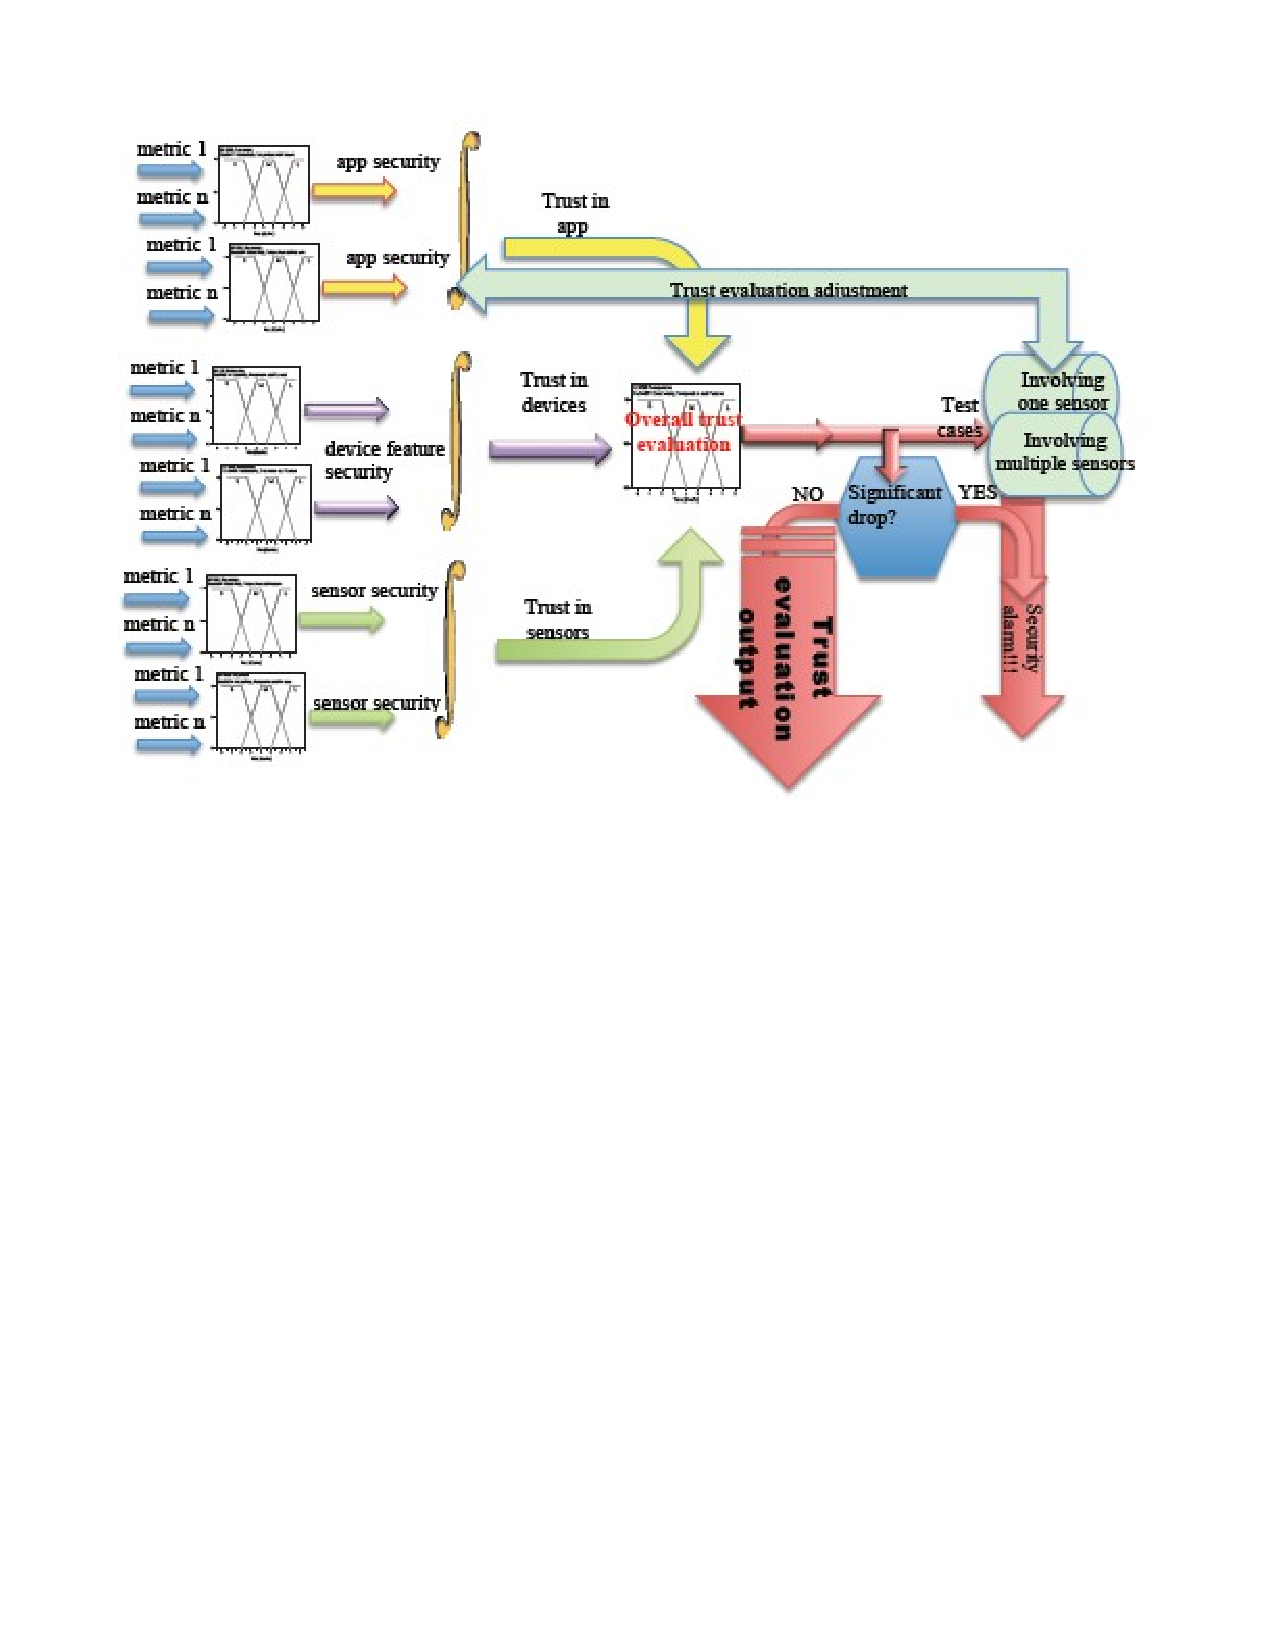
\includegraphics[width=3.5in]{umbrella_framework.pdf}
\caption{Framework operation and architecture.}
\label{fig:umbrella}
\end{figure}

